\chapter*{Proposition 26}

\begin{figure*}[ht]
    \begin{center}
    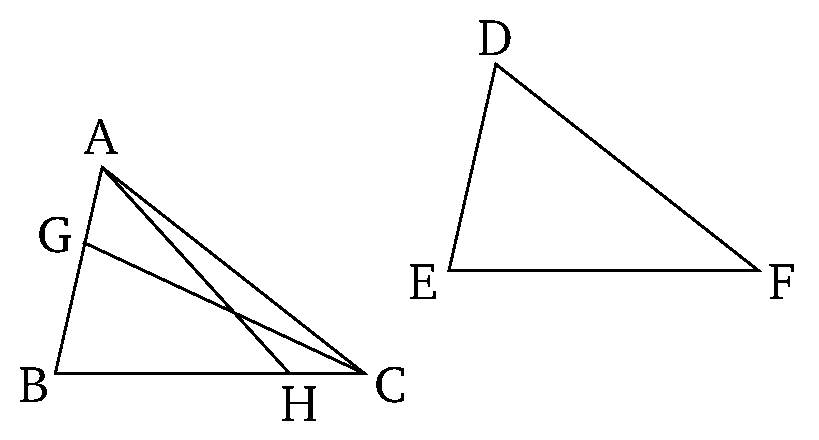
\includegraphics[width=0.5\linewidth]{figures/fig26e.eps}
    \label{fig:prop_26}
    \end{center}
\end{figure*}


If  two triangles have two angles equal to two angles, respectively, 
and one side equal to one side---in fact, either that by the equal angles, or that
subtending one of the equal angles---then (the triangles) will also have the remaining
sides equal to the [corresponding] remaining sides, and the
remaining angle (equal) to the remaining angle.

Let $ABC$ and $DEF$ be two triangles having the two angles $ABC$ and
$BCA$ equal to the two (angles) $DEF$ and $EFD$, respectively.
(That is) $ABC$ (equal) to $DEF$, and $BCA$ to $EFD$. And let them also have
one side equal to one side. First of all, the (side) by the equal angles. (That is)
$BC$ (equal) to $EF$. I say that they will have the  remaining sides equal to the
corresponding remaining sides. (That is) $AB$ (equal) to $DE$, and $AC$ to
$DF$. And (they will have) the remaining angle (equal) to the remaining angle.
(That is) $BAC$ (equal) to $EDF$.

For if $AB$ is unequal to $DE$ then one of them is greater. Let $AB$ be greater,
and let $BG$ be made equal to $DE$ [Prop.~1.3], and let $GC$ have been
joined.

Therefore, since $BG$ is equal to $DE$, and $BC$ to $EF$, the two (straight-lines)
$GB$, $BC$ are equal to the two (straight-lines) $DE$, $EF$, respectively. And angle
$GBC$ is equal to angle $DEF$. Thus, the base $GC$ is equal to the base $DF$,
and triangle $GBC$ is equal to triangle $DEF$, and the remaining angles 
subtended by the equal sides will
be equal to the (corresponding) remaining angles [Prop.~1.4].
Thus, $GCB$ (is equal) to $DFE$. But,  $DFE$ was assumed (to be) equal to $BCA$.
Thus, $BCG$ is also equal to $BCA$, the lesser to the greater. The very thing (is) impossible. Thus, $AB$ is not unequal to $DE$. Thus, (it is) equal. And $BC$ is
also equal to $EF$. So the two (straight-lines) $AB$, $BC$ are equal to the two (straight-lines) $DE$, $EF$, respectively. And angle $ABC$ is equal to
angle $DEF$. Thus, the base $AC$ is equal to the base $DF$, and the remaining
angle $BAC$ is equal to the remaining angle $EDF$ [Prop.~1.4].

But, again, let the sides subtending the equal angles be equal: for instance, 
(let) $AB$ (be equal) to
$DE$.  Again, I say that the remaining sides will be equal to the remaining
sides. (That is) $AC$ (equal) to $DF$, and $BC$ to $EF$. Furthermore, the remaining angle
$BAC$ is equal to the remaining angle $EDF$.

For if $BC$ is unequal to $EF$ then one of them is greater. If possible, let $BC$
be greater. And let $BH$ be made equal to $EF$ [Prop.~1.3], and let $AH$ have been joined.
And since $BH$ is equal to $EF$, and $AB$ to $DE$, the two (straight-lines) $AB$, $BH$
are equal to the two (straight-lines) $DE$, $EF$, respectively. And the angles
they encompass (are also equal). Thus, the base $AH$ is equal to the base  
$DF$, and the triangle $ABH$ is equal to the triangle $DEF$, and the
remaining angles subtended by the equal sides will be equal to the
(corresponding) remaining angles [Prop.~1.4]. Thus, angle $BHA$ 
is equal to $EFD$. But, $EFD$ is equal to $BCA$. So, in triangle $AHC$,
the external angle $BHA$ is equal to the internal and opposite angle 
$BCA$. The very thing (is) impossible [Prop.~1.16]. Thus, $BC$ is not unequal to $EF$.
Thus, (it is) equal. And $AB$ is also equal to $DE$. So the two
(straight-lines) $AB$, $BC$ are equal to the two (straight-lines) $DE$, $EF$,
respectively. And they encompass equal angles. Thus, the base $AC$ is equal
to the base $DF$, and triangle $ABC$ (is) equal to triangle $DEF$, and the
remaining angle $BAC$ (is) equal to the remaining angle $EDF$ [Prop.~1.4].

Thus, if two triangles have two angles equal to two angles, respectively, 
and one side equal to one side---in fact, either that by the equal angles, or that
subtending one of the equal angles---then (the triangles) will also have the remaining sides equal to the (corresponding) remaining sides, and the
remaining angle (equal) to the remaining angle. (Which is) the very thing it
was required to show.



\section*{Commentary}

\begin{proposition}\label{proposition_26}\lean{Elements.Book1.proposition_26}\leanok
    $\triangle~ABC$ and $\triangle~DEF$ are two triangles, s.t., $\angle~ABC=\angle~DEF$, $\angle~BCA=\angle~EFD$, and $|BC|=|EF|$ (or $|AB|=|DE|$). Then, $\triangle~ABC\cong\triangle~DEF$.
\end{proposition}
\begin{proof}
    \uses{proposition_3,proposition_4,proposition_16}\leanok
    See the original proof by Euclid.
\end{proof}
